% Generated by pysimcount.pfboundratio -- do not edit; regenerate instead.
% figure: bound-ratio-suzuki6 -- Suzuki S6: Trotter number from each bound / measured r, against n
% metric=r_ratio gatebase=cz; geometric mean over seeds [1, 2, 3, 4, 5, 6, 7, 8, 9, 10], bars min-max; r_method=measured (denominator); bounds: Analytic bound, Minimised bound, Commutator bound (2018), Commutator bound (2021), Empirical fit (2018)
% sizes: np-main n = [4, 5, 6, 7, 8, 10]; np-main-n9 n = [9]; np-main-n11 n = [11]
% run set np-main-n9 made from uncommitted code (git_dirty), accepted: run at e42ff29 with the only modified tracked file pysimcount/pfseeds.py (an aggregation module the run does not import); checked with git diff --stat e42ff29 -- pysimcount/ on 2026-11-08
% run set np-main-n11 made from uncommitted code (git_dirty), accepted: run at e42ff29 with the only modified tracked file pysimcount/pfseeds.py (an aggregation module the run does not import); checked with git diff --stat e42ff29 -- pysimcount/ on 2026-11-08
% formulas: Suzuki S6
% figure made at git_commit=e5d9ee696f892e28aced765585653760f8a427c4 git_dirty=False
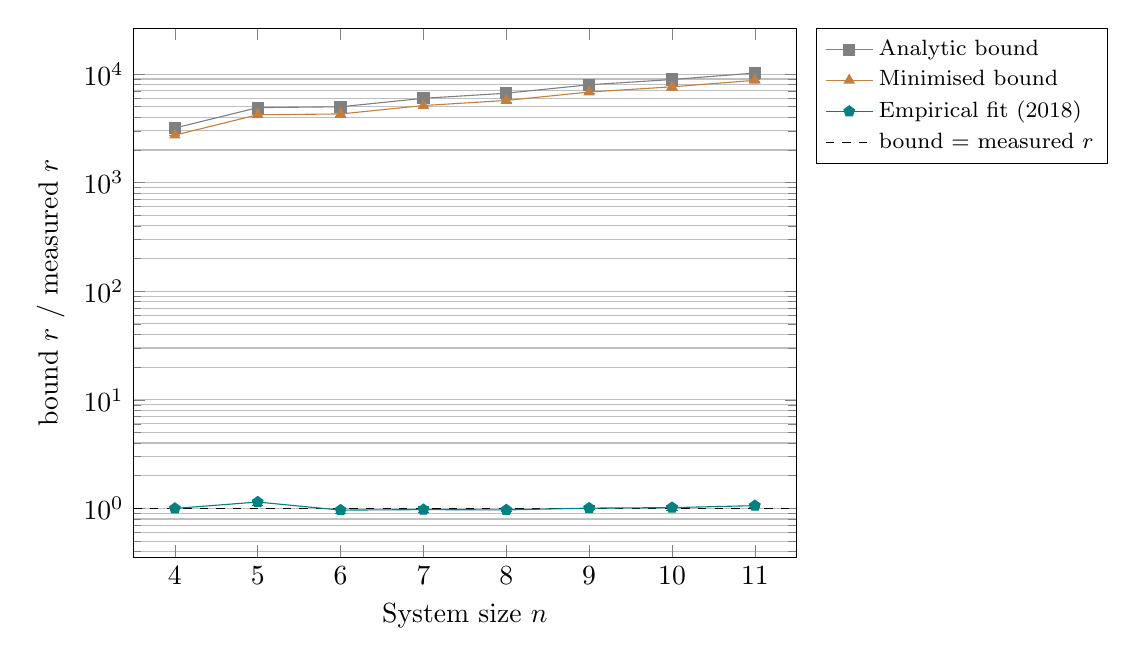
\begin{tikzpicture}
  \begin{semilogyaxis}[
    width=10cm, height=8.3cm,
    xlabel={System size $n$}, ylabel={bound $r$ / measured $r$},
    xmin=3.5, xmax=11.5,
    xtick={4,5,6,7,8,9,10,11},
    ymajorgrids=true, yminorgrids=true,
    legend pos=outer north east, legend cell align=left,
    legend style={font=\footnotesize},
  ]
    \addplot[dashed, black, domain=3.5:11.5, samples=2, forget plot] {1};
    \addplot[solid, gray, mark=square*, mark size=2pt, error bars/.cd, y dir=both, y explicit] coordinates {
      (4,3184.42) -= (0,-1.81899e-12) += (0,1.81899e-12)
      (5,4911.01) -= (0,316.866) += (0,36.5297)
      (6,4998.61) -= (0,311.897) += (0,181.441)
      (7,5979.06) -= (0,338.098) += (0,431.124)
      (8,6664.79) -= (0,245.492) += (0,213.029)
      (9,7974.47) -= (0,292.898) += (0,475.26)
      (10,8909.7) -= (0,598.447) += (0,351.411)
      (11,10225.4) -= (0,350.535) += (0,155.867)
    };
    \addlegendentry{Analytic bound}
    \addplot[solid, brown, mark=triangle*, mark size=2pt, error bars/.cd, y dir=both, y explicit] coordinates {
      (4,2739.67) -= (0,-4.54747e-13) += (0,4.54747e-13)
      (5,4220.22) -= (0,272.295) += (0,31.3914)
      (6,4291.74) -= (0,267.791) += (0,155.783)
      (7,5129.96) -= (0,290.085) += (0,369.899)
      (8,5714.97) -= (0,210.506) += (0,182.67)
      (9,6834.67) -= (0,251.033) += (0,407.33)
      (10,7632.97) -= (0,512.691) += (0,301.055)
      (11,8756.88) -= (0,300.193) += (0,133.483)
    };
    \addlegendentry{Minimised bound}
    \addplot[solid, teal, mark=pentagon*, mark size=2pt, error bars/.cd, y dir=both, y explicit] coordinates {
      (4,1) -= (0,0) += (0,0)
      (5,1.14533) -= (0,0.0738983) += (0,0.00851931)
      (6,0.964973) -= (0,0.0602113) += (0,0.0350268)
      (7,0.975141) -= (0,0.0551414) += (0,0.0703131)
      (8,0.969027) -= (0,0.0356933) += (0,0.0309734)
      (9,1.00667) -= (0,0.0369744) += (0,0.0599953)
      (10,1.01703) -= (0,0.0683118) += (0,0.0401131)
      (11,1.06075) -= (0,0.0363636) += (0,0.0161693)
    };
    \addlegendentry{Empirical fit (2018)}
    \addlegendimage{dashed, black}
    \addlegendentry{bound $=$ measured $r$}
  \end{semilogyaxis}
\end{tikzpicture}
